\documentclass[11pt]{article}
\usepackage{minted, tikz}
\usepackage{amsfonts, amssymb, amsmath, float}
\usepackage{enumerate, esint, nicefrac, algorithm2e}
\parindent 0px
\date{September 20, 2023}
\title{CS301 :: Homework 2}
\author{Ryan Magdaleno}

% Helpful ::
% \line(1,0){358px}

\begin{document}
\maketitle

%%%%%%%%%%%%%%%%%%%%%%%%%%%%%%%%%%%%%%%%%%%%%%%%%%%%%%%%%%%%%%%%%%%%%%%%%%%%%%%%%%%%%%%%%

\textbf{Problem 1. NFA to DFA}

Prove the state diagram for a DFA that accepts the same language as the NFA $M$ below.
You do \textbf{not} need to provide the 5-tuple.

\begin{center}
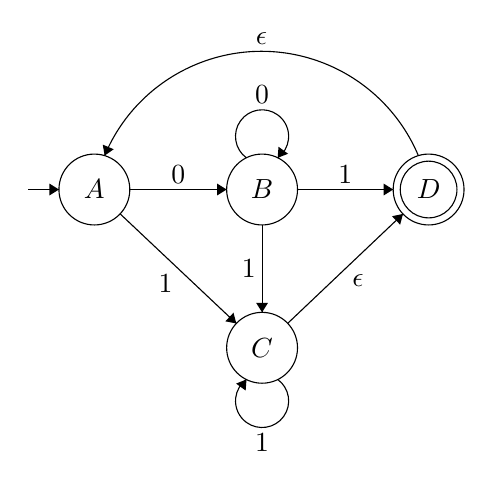
\begin{tikzpicture}[scale=0.15]
\tikzstyle{every node}+=[inner sep=0pt]
\draw [black] (20.9,-19.7) circle (3);
\draw (20.9,-19.7) node {$A$};
\draw [black] (35.1,-19.7) circle (3);
\draw (35.1,-19.7) node {$B$};
\draw [black] (35.1,-33.1) circle (3);
\draw (35.1,-33.1) node {$C$};
\draw [black] (49.2,-19.7) circle (3);
\draw (49.2,-19.7) node {$D$};
\draw [black] (49.2,-19.7) circle (2.4);
\draw [black] (37.27,-31.03) -- (47.03,-21.77);
\fill [black] (47.03,-21.77) -- (46.1,-21.96) -- (46.79,-22.68);
\draw (43.22,-26.88) node [below] {$\epsilon$};
\draw [black] (35.1,-22.7) -- (35.1,-30.1);
\fill [black] (35.1,-30.1) -- (35.6,-29.3) -- (34.6,-29.3);
\draw (34.6,-26.4) node [left] {$1$};
\draw [black] (23.08,-21.76) -- (32.92,-31.04);
\fill [black] (32.92,-31.04) -- (32.68,-30.13) -- (31.99,-30.86);
\draw (26.93,-26.88) node [below] {$1$};
\draw [black] (36.423,-35.78) arc (54:-234:2.25);
\draw (35.1,-40.35) node [below] {$1$};
\fill [black] (33.78,-35.78) -- (32.9,-36.13) -- (33.71,-36.72);
\draw [black] (38.1,-19.7) -- (46.2,-19.7);
\fill [black] (46.2,-19.7) -- (45.4,-19.2) -- (45.4,-20.2);
\draw (42.15,-19.2) node [above] {$1$};
\draw [black] (23.9,-19.7) -- (32.1,-19.7);
\fill [black] (32.1,-19.7) -- (31.3,-19.2) -- (31.3,-20.2);
\draw (28,-19.2) node [above] {$0$};
\draw [black] (33.777,-17.02) arc (234:-54:2.25);
\draw (35.1,-12.45) node [above] {$0$};
\fill [black] (36.42,-17.02) -- (37.3,-16.67) -- (36.49,-16.08);
\draw [black] (21.765,-16.833) arc (157.24397:22.75603:14.406);
\fill [black] (21.77,-16.83) -- (22.54,-16.29) -- (21.61,-15.9);
\draw (35.05,-7.5) node [above] {$\epsilon$};
\draw [black] (15.3,-19.7) -- (17.9,-19.7);
\fill [black] (17.9,-19.7) -- (17.1,-19.2) -- (17.1,-20.2);
\end{tikzpicture}
\end{center}

\vspace{5px}\textbf{Solution ::}

\begin{center}
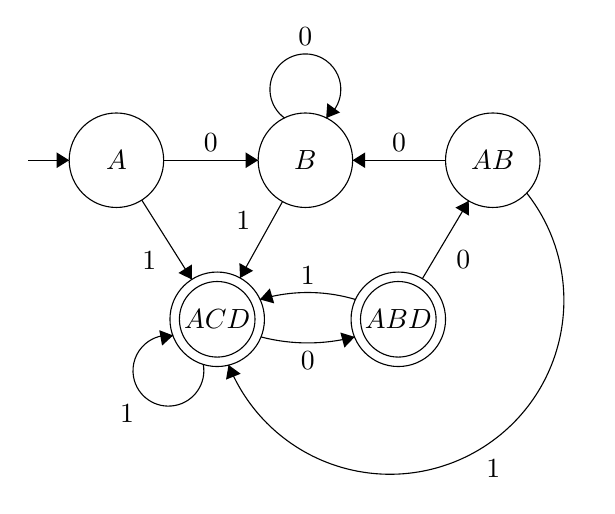
\begin{tikzpicture}[scale=0.2]
\tikzstyle{every node}+=[inner sep=0pt]
\draw [black] (12.6,-15.8) circle (3);
\draw (12.6,-15.8) node {$A$};
\draw [black] (24.6,-15.8) circle (3);
\draw (24.6,-15.8) node {$B$};
\draw [black] (19,-25.9) circle (3);
\draw (19,-25.9) node {$ACD$};
\draw [black] (19,-25.9) circle (2.4);
\draw [black] (30.5,-25.9) circle (3);
\draw (30.5,-25.9) node {$ABD$};
\draw [black] (30.5,-25.9) circle (2.4);
\draw [black] (36.5,-15.8) circle (3);
\draw (36.5,-15.8) node {$AB$};
\draw [black] (15.6,-15.8) -- (21.6,-15.8);
\fill [black] (21.6,-15.8) -- (20.8,-15.3) -- (20.8,-16.3);
\draw (18.6,-15.3) node [above] {$0$};
\draw [black] (23.277,-13.12) arc (234:-54:2.25);
\draw (24.6,-8.55) node [above] {$0$};
\fill [black] (25.92,-13.12) -- (26.8,-12.77) -- (25.99,-12.18);
\draw [black] (14.21,-18.33) -- (17.39,-23.37);
\fill [black] (17.39,-23.37) -- (17.39,-22.42) -- (16.54,-22.96);
\draw (15.17,-22.15) node [left] {$1$};
\draw [black] (23.15,-18.42) -- (20.45,-23.28);
\fill [black] (20.45,-23.28) -- (21.28,-22.82) -- (20.41,-22.33);
\draw (21.13,-19.65) node [left] {$1$};
\draw [black] (27.725,-27.019) arc (-75.35135:-104.64865:11.764);
\fill [black] (27.73,-27.02) -- (26.82,-26.74) -- (27.08,-27.7);
\draw (24.75,-27.9) node [below] {$0$};
\draw [black] (18.114,-28.754) arc (10.4803:-277.5197:2.25);
\draw (13.28,-31.28) node [below] {$1$};
\fill [black] (16.2,-26.93) -- (15.32,-26.59) -- (15.5,-27.57);
\draw [black] (33.5,-15.8) -- (27.6,-15.8);
\fill [black] (27.6,-15.8) -- (28.4,-16.3) -- (28.4,-15.3);
\draw (30.55,-15.3) node [above] {$0$};
\draw [black] (32.03,-23.32) -- (34.97,-18.38);
\fill [black] (34.97,-18.38) -- (34.13,-18.81) -- (34.99,-19.32);
\draw (34.15,-22.11) node [right] {$0$};
\draw [black] (38.651,-17.878) arc (38.19203:-158.20986:11.039);
\fill [black] (19.72,-28.8) -- (19.56,-29.73) -- (20.49,-29.36);
\draw (36.54,-34.77) node [below] {$1$};
\draw [black] (7,-15.8) -- (9.6,-15.8);
\fill [black] (9.6,-15.8) -- (8.8,-15.3) -- (8.8,-16.3);
\draw [black] (21.714,-24.645) arc (106.69657:73.30343:10.569);
\fill [black] (21.71,-24.64) -- (22.62,-24.89) -- (22.34,-23.94);
\draw (24.75,-23.7) node [above] {$1$};
\end{tikzpicture}
\end{center}

\pagebreak

%%%%%%%%%%%%%%%%%%%%%%%%%%%%%%%%%%%%%%%%%%%%%%%%%%%%%%%%%%%%%%%%%%%%%%%%%%%%%%%%%%%%%%%%%

\textbf{Problem 2. Regular Expression to NFA} 

Produce the state diagram for a NFA which decides the following languages. \\
$\sum=\{a,b,c\}$ \textit{You do not need to produce the 5-tuple.}

\begin{enumerate}[a)]
    \item 
    $L_a = (abc)^*\cup (ab)^*$ \\
    \vspace{5px}\textbf{Solution ::}
    \begin{center}
    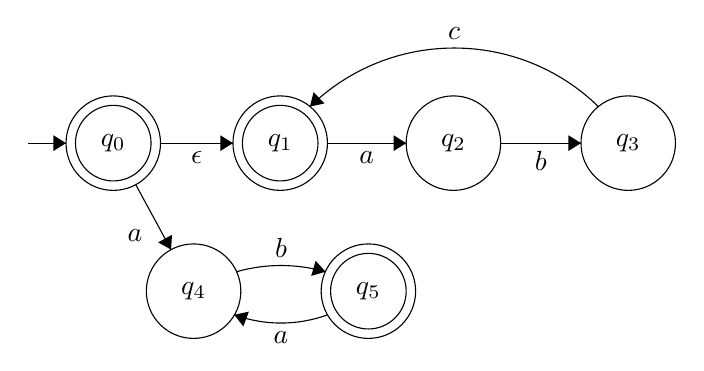
\begin{tikzpicture}[scale=0.2]
    \tikzstyle{every node}+=[inner sep=0pt]
    \draw [black] (17.5,-20.2) circle (3);
    \draw (17.5,-20.2) node {$q_0$};
    \draw [black] (17.5,-20.2) circle (2.4);
    \draw [black] (28.1,-20.2) circle (3);
    \draw (28.1,-20.2) node {$q_1$};
    \draw [black] (28.1,-20.2) circle (2.4);
    \draw [black] (39.1,-20.2) circle (3);
    \draw (39.1,-20.2) node {$q_2$};
    \draw [black] (50.2,-20.2) circle (3);
    \draw (50.2,-20.2) node {$q_3$};
    \draw [black] (22.6,-29.6) circle (3);
    \draw (22.6,-29.6) node {$q_4$};
    \draw [black] (33.7,-29.6) circle (3);
    \draw (33.7,-29.6) node {$q_5$};
    \draw [black] (33.7,-29.6) circle (2.4);
    \draw [black] (20.5,-20.2) -- (25.1,-20.2);
    \fill [black] (25.1,-20.2) -- (24.3,-19.7) -- (24.3,-20.7);
    \draw (22.8,-20.7) node [below] {$\epsilon$};
    \draw [black] (18.93,-22.84) -- (21.17,-26.96);
    \fill [black] (21.17,-26.96) -- (21.23,-26.02) -- (20.35,-26.5);
    \draw (19.38,-26.08) node [left] {$a$};
    \draw [black] (25.323,-28.367) arc (105.98292:74.01708:10.266);
    \fill [black] (30.98,-28.37) -- (30.35,-27.67) -- (30.07,-28.63);
    \draw (28.15,-27.47) node [above] {$b$};
    \draw [black] (31.118,-31.098) arc (-69.85833:-110.14167:8.619);
    \fill [black] (25.18,-31.1) -- (25.76,-31.84) -- (26.11,-30.9);
    \draw (28.15,-32.12) node [below] {$a$};
    \draw [black] (31.1,-20.2) -- (36.1,-20.2);
    \fill [black] (36.1,-20.2) -- (35.3,-19.7) -- (35.3,-20.7);
    \draw (33.6,-20.7) node [below] {$a$};
    \draw [black] (42.1,-20.2) -- (47.2,-20.2);
    \fill [black] (47.2,-20.2) -- (46.4,-19.7) -- (46.4,-20.7);
    \draw (44.65,-20.7) node [below] {$b$};
    \draw [black] (29.993,-17.881) arc (134.22929:45.77071:13.128);
    \fill [black] (29.99,-17.88) -- (30.91,-17.68) -- (30.22,-16.96);
    \draw (39.15,-13.66) node [above] {$c$};
    \draw [black] (12.1,-20.2) -- (14.5,-20.2);
    \fill [black] (14.5,-20.2) -- (13.7,-19.7) -- (13.7,-20.7);
    \end{tikzpicture}
    \end{center}

    \line(1,0){343px}

    \item
    $L_b = ((ab)^*c)^*$ \\
    \vspace{5px}\textbf{Solution ::}
    \begin{center}
    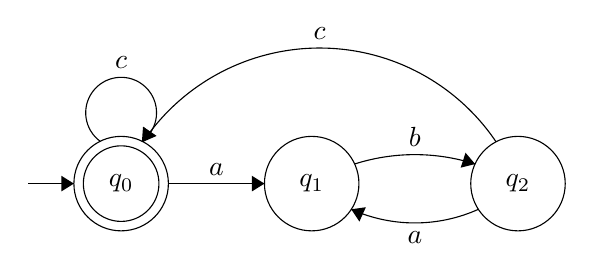
\begin{tikzpicture}[scale=0.2]
    \tikzstyle{every node}+=[inner sep=0pt]
    \draw [black] (19,-25.8) circle (3);
    \draw (19,-25.8) node {$q_0$};
    \draw [black] (19,-25.8) circle (2.4);
    \draw [black] (31.1,-25.8) circle (3);
    \draw (31.1,-25.8) node {$q_1$};
    \draw [black] (44.2,-25.8) circle (3);
    \draw (44.2,-25.8) node {$q_2$};
    \draw [black] (13.1,-25.8) -- (16,-25.8);
    \fill [black] (16,-25.8) -- (15.2,-25.3) -- (15.2,-26.3);
    \draw [black] (22,-25.8) -- (28.1,-25.8);
    \fill [black] (28.1,-25.8) -- (27.3,-25.3) -- (27.3,-26.3);
    \draw (25.05,-25.3) node [above] {$a$};
    \draw [black] (33.822,-24.556) arc (107.73003:72.26997:12.57);
    \fill [black] (41.48,-24.56) -- (40.87,-23.84) -- (40.56,-24.79);
    \draw (37.65,-23.46) node [above] {$b$};
    \draw [black] (41.694,-27.428) arc (-65.7261:-114.2739:9.837);
    \fill [black] (33.61,-27.43) -- (34.13,-28.21) -- (34.54,-27.3);
    \draw (37.65,-28.8) node [below] {$a$};
    \draw [black] (20.39,-23.148) arc (145.9786:34.0214:13.525);
    \fill [black] (20.39,-23.15) -- (21.25,-22.77) -- (20.42,-22.21);
    \draw (31.6,-16.69) node [above] {$c$};
    \draw [black] (17.677,-23.12) arc (234:-54:2.25);
    \draw (19,-18.55) node [above] {$c$};
    \fill [black] (20.32,-23.12) -- (21.2,-22.77) -- (20.39,-22.18);
    \end{tikzpicture}
    \end{center}
\end{enumerate}

\pagebreak

%%%%%%%%%%%%%%%%%%%%%%%%%%%%%%%%%%%%%%%%%%%%%%%%%%%%%%%%%%%%%%%%%%%%%%%%%%%%%%%%%%%%%%%%%

\textbf{Problem 3. NFA to Regular Expressions}

Give a regular expression for the language decided by the following NFA $M$. 
\\ Let $\sum = \{0,1\}$ \\
Show the intermediate GNFAs after removing each state.

\begin{center}
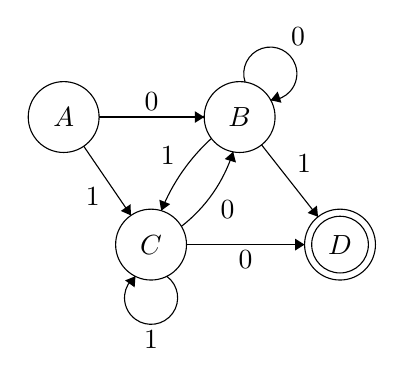
\begin{tikzpicture}[scale=0.15]
\tikzstyle{every node}+=[inner sep=0pt]
\draw [black] (19.5,-17.2) circle (3);
\draw (19.5,-17.2) node {$A$};
\draw [black] (34.4,-17.2) circle (3);
\draw (34.4,-17.2) node {$B$};
\draw [black] (26.9,-28) circle (3);
\draw (26.9,-28) node {$C$};
\draw [black] (42.9,-28) circle (3);
\draw (42.9,-28) node {$D$};
\draw [black] (42.9,-28) circle (2.4);
\draw [black] (22.5,-17.2) -- (31.4,-17.2);
\fill [black] (31.4,-17.2) -- (30.6,-16.7) -- (30.6,-17.7);
\draw (26.95,-16.7) node [above] {$0$};
\draw [black] (21.2,-19.67) -- (25.2,-25.53);
\fill [black] (25.2,-25.53) -- (25.16,-24.58) -- (24.34,-25.15);
\draw (22.6,-23.95) node [left] {$1$};
\draw [black] (28.223,-30.68) arc (54:-234:2.25);
\draw (26.9,-35.25) node [below] {$1$};
\fill [black] (25.58,-30.68) -- (24.7,-31.03) -- (25.51,-31.62);
\draw [black] (29.9,-28) -- (39.9,-28);
\fill [black] (39.9,-28) -- (39.1,-27.5) -- (39.1,-28.5);
\draw (34.9,-28.5) node [below] {$0$};
\draw [black] (27.762,-25.131) arc (158.12173:132.32261:16.69);
\fill [black] (27.76,-25.13) -- (28.52,-24.57) -- (27.6,-24.2);
\draw (28.94,-20.47) node [left] {$1$};
\draw [black] (33.851,-20.142) arc (-17.28871:-52.26695:12.792);
\fill [black] (33.85,-20.14) -- (33.14,-20.76) -- (34.09,-21.05);
\draw (32.74,-25) node [right] {$0$};
\draw [black] (36.26,-19.56) -- (41.04,-25.64);
\fill [black] (41.04,-25.64) -- (40.94,-24.7) -- (40.16,-25.32);
\draw (39.22,-21.18) node [right] {$1$};
\draw [black] (34.866,-14.248) arc (198.75878:-89.24122:2.25);
\draw (39.35,-11.19) node [above] {$0$};
\fill [black] (37.03,-15.77) -- (37.94,-15.99) -- (37.62,-15.04);
\end{tikzpicture}
\end{center}

\vspace{5px}\textbf{Solution ::}

\textbf{Removing State B ::}
\begin{center}
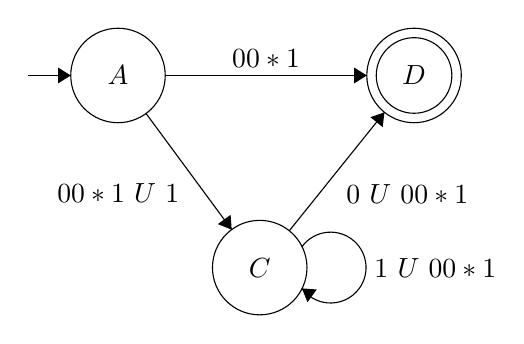
\begin{tikzpicture}[scale=0.2]
\tikzstyle{every node}+=[inner sep=0pt]
\draw [black] (25.1,-14.7) circle (3);
\draw (25.1,-14.7) node {$A$};
\draw [black] (43.9,-14.7) circle (3);
\draw (43.9,-14.7) node {$D$};
\draw [black] (43.9,-14.7) circle (2.4);
\draw [black] (34.1,-26.9) circle (3);
\draw (34.1,-26.9) node {$C$};
\draw [black] (19.4,-14.7) -- (22.1,-14.7);
\fill [black] (22.1,-14.7) -- (21.3,-14.2) -- (21.3,-15.2);
\draw [black] (28.1,-14.7) -- (40.9,-14.7);
\fill [black] (40.9,-14.7) -- (40.1,-14.2) -- (40.1,-15.2);
\draw (34.5,-14.2) node [above] {$00*1$};
\draw [black] (26.88,-17.11) -- (32.32,-24.49);
\fill [black] (32.32,-24.49) -- (32.25,-23.55) -- (31.44,-24.14);
\draw (29.02,-22.19) node [left] {$00*1\mbox{ }U\mbox{ }1$};
\draw [black] (36.78,-25.577) arc (144:-144:2.25);
\draw (41.35,-26.9) node [right] {$1\mbox{ }U\mbox{ }00*1$};
\fill [black] (36.78,-28.22) -- (37.13,-29.1) -- (37.72,-28.29);
\draw [black] (35.98,-24.56) -- (42.02,-17.04);
\fill [black] (42.02,-17.04) -- (41.13,-17.35) -- (41.91,-17.98);
\draw (39.56,-22.22) node [right] {$0\mbox{ }U\mbox{ }00*1$};
\end{tikzpicture}
\end{center}

\textbf{Removing state C ::}
\begin{center}
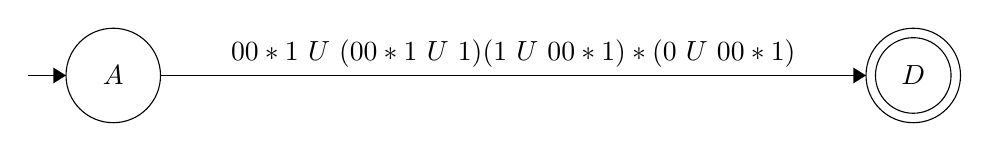
\begin{tikzpicture}[scale=0.2]
\tikzstyle{every node}+=[inner sep=0pt]
\draw [black] (15.9,-16) circle (3);
\draw (15.9,-16) node {$A$};
\draw [black] (66.7,-16) circle (3);
\draw (66.7,-16) node {$D$};
\draw [black] (66.7,-16) circle (2.4);
\draw [black] (18.9,-16) -- (63.7,-16);
\fill [black] (63.7,-16) -- (62.9,-15.5) -- (62.9,-16.5);
\draw (41.3,-15.5) node [above] {$00*1\mbox{ }U\mbox{ }
(00*1\mbox{ }U\mbox{ }1)(1\mbox{ }U\mbox{ }00*1)*(0\mbox{ }U\mbox{ }00*1)$};
\draw [black] (10.5,-16) -- (12.9,-16);
\fill [black] (12.9,-16) -- (12.1,-15.5) -- (12.1,-16.5);
\end{tikzpicture}
\end{center}
\end{document}